
\section{Analysis: RMSE vs Spike Rate for a Fixed Dynamical System}


 Here we derive the RMSE of a signal representing a given dynamical system with a varying spike rate. The RMSE is computed over a constant interval of time for a fixed target system while the spike rate is varied.  
\begin{enumerate}
\item Our system is described by 

\begin{align*}
A &= -\begin{bmatrix}  
1 & 0 \\
0 & 1
\end{bmatrix},\notag \\
\notag \\
B &= \begin{bmatrix}  
1 & 0 \\
0 & 1
\end{bmatrix}, \notag \\
\notag \\
c(\xi) &= \mathcal{U}_1 \\
\notag \\
d\xi &= 10^{-4},\notag \\
\notag \\
N &= 4,\notag \\
\notag \\
x(0) &= \begin{bmatrix} \frac{1}{2} & 0 \end{bmatrix}.\notag 
\end{align*}

\item With the given initial conditions, $v_j = 0$ for $j \neq 1$ for all $\xi$. From equations (\ref{eq:rotated_voltage_psc_def}) and (\ref{eq:rotated_voltage_dynamics}), the dynamics simplify to 
\begin{equation*}
\dot{v_1} = \Lambda_1 v_1 + (\Lambda_1 + 1)\rho_1 + S_1 \mathcal{U}_1^T \mathcal{U}_1 - \Omega_1.
\end{equation*}

It is clear that $\Lambda_1 = -1$ so that 
\begin{equation}
\label{eq:analysis_voltage_dynamics_constant_driving_const_dynamics}
\dot{v_1} = -v_1 + S_1 - \Omega_1,
\end{equation}
which is a form of the well-known Leaky Integrate-and-Fire (LIF) model.
\item  Assuming a spike has occurred at $v_{th} = \frac{1}{2}$, the voltage has just been reset so that $v_1(0) = -\frac{1}{2}$. Until the next spike, the neuron's trajectory is integrated as 
\begin{align*}
v(\xi) =  S_1 - e^{-\xi} (S_1 + \frac{1}{2}).
\end{align*}

The spike occurs at $v(\xi_{spike}) = v_{th}$ or 
\begin{align*}
v_{th} &= S_1 - e^
{
	-\xi
}
(
	S_1 + \frac		
		  {
			  1
		  }
		  {
			  2
		  }
 ) 
%
\\
\\
%
\implies 
\frac
{
	S_1 - v_{th}  
}
{
	S_1 + \frac
		  {
		       1
		  }
		  {
		  	   2
		  }
}
&=
e^
{
	-\xi_{spike}
}
%
\\
\\
%
\implies
\xi_{spike}
&= 
ln
(
	S_1 + \frac
			{
				1
			}
			{
				2
			}
)
- 
ln
(
	S_1 - v_{th}
).
\end{align*}

The inverse of the preceding expression gives the firing rate of the neuron,

\begin{align}
\label{eq:analysis_const_dynamics_phi_vs_s}
\phi(S_1)
\overset{\Delta}{=}
\frac
{
	1
} 
{
	ln
	(
		1 + \frac
				{
					1
				}
				{
					2 \, S_1
				}
	)
	- 
	ln
	(
		1 - \frac
			{
				v_{th}
			}
			{
				S_1
			}
	)
}.
\end{align}

Equation (\ref{eq:analysis_const_dynamics_phi_vs_s}) describes the neuron's firing rate as a function of the decode matrix $D$'s singular values. Thus for a given target dynamical system, the decode matrix $D$ determines the neuron's firing rates. 

\item From equations (\ref{eq:rho_dot}), (\ref{eq:xhat}), and (\ref{eq:delta_dec}),
\begin{align}
\label{eq:analysis:constant_driving_constant_dynamics_estimate_equation_implicit}
\dot
{
	\rho
}
&= 	- \rho  + \Omega \notag
% 
\\ \notag
\\ \notag
%
\implies
\dot{
	\hat
	{
		x
	}
}
&= 
-\hat
{
	x
}
+ \Delta \Omega
% \notag
\\ \notag
\\ 
%
\implies
\dot
{
	\hat
	{
		x
	}
}
&= 
-\hat
{
	x
}
+ S_1^
{
	-1
}
\mathcal
{
	U
}_1 
\sum_
{
	l=0
}
^
{
	\infty
}
\delta 
\left(
	\xi - \frac
		  {
			  l
		  }
		  {
			  \phi
		  }
\right),
\end{align}
where the last equality follows from the periodicity of the LIF neuron firing at rate $\phi$.

We solve equation (\ref{eq:analysis:constant_driving_constant_dynamics_estimate_equation_implicit}) and inductively derive an explicit expression for its asymptotic behavior in time. Note that equation (\ref{eq:analysis:constant_driving_constant_dynamics_estimate_equation_implicit}) implies that the network estimate $\hat{x}$ will decay until the first spike $\xi_1^1$ occurs:
\begin{align*}
\hat{x}(\xi) = x(0) e^{-\xi}, \hspace{4mm} 0 \leq \xi < \xi_1^1.
\end{align*}


 At this instant, the scaled vector $ S_1^{-1} \mathcal{U}_1$ is added to the network estimate,
 \begin{align*}
 \hat{x}( \xi_1^1) =  x(0) e^{-\xi_1^1 } + S_1^{-1}\mathcal{U}_1.
 \end{align*}
 
Decay again occurs until the next spike
\begin{align*}
\hat{
	x
}
(
	\xi
)
&= \hat
{
	x
}
(
	\xi_{1}^1
)
e^
{
	-
	(
		\xi - \xi_{1}^1
	)
},
%
\\
\\
%
&=
\left(
	 x(0) e^
	 {
	 	-\xi_1^1
	 }
	 + S_1^
	 {
	 	-1
	 }
	 \mathcal{U}_1
\right)
e^
{
	-
	(
		\xi - 
		\xi_1^1
	)
} , \hspace{4mm} 
0 \leq \xi - \xi_1^1 <
\frac
{
	1
}
{
	\phi
}
%
\\
\\
%
\implies
\hat
{
	x
}
(
	\xi_1^1 + 
	\frac
	{
		1
	}
	{
		\phi
	}
)
&=
\left(
	x
	(
		0
	)
	e^
	{
		- \xi_1^1
	}
	 + S_1^
	 {
	 	-1
	 }
	 \mathcal{U}_1 
\right)
e^
{
	-
	\frac
	{
		1
	}
	{
		\phi
	}
}
+ S_1^
{
	-1
}
\mathcal{U}_1
\\
\\
&=
x
(
	0
)
e^
{	
	-\left(
		\xi_1^1 + 
		\frac
		{
			1
		}
		{
			\phi
		}
	\right)
}
+ S_1^
{
	-1
}
\mathcal{U}_1
e^
{
	-\frac
	{
		1
	}
	{
		\phi
	}
} 
+ S_1^
{
	-1
}
\mathcal{U}_1.
\end{align*}

The third spike more clearly shows the recursive behavior
\begin{align*}
\hat
{
	x
}
(
	\xi_1^1 + 
	\frac
	{
		2
	}
	{
		\phi
	}
)
&= 
\left[
	x
	(
		0
	)
	e^
	{	
		-\left(
			\xi_1^1 + 
			\frac
			{
				1
			}
			{
				\phi
			}
		\right)
	}
	+ S_1^
	{
		-1
	}
	\mathcal{U}_1
	e^
	{
		-\frac
		{
			1
		}
		{
			\phi
		}
	} 
	+ S_1^
	{
		-1
	}
	\mathcal{U}_1.
\right]
e^
{
	-\frac
	{
		1
	}
	{
			\phi
	}
}
+ S_1^
{
	-1
}
\mathcal{U}_1 
%
\\
\\
%
&= 
x
(
	0
)
e^
{	
	-\left(
		\xi_1^1 + 
		\frac
		{
			2
		}
		{
			\phi
		}
	\right)
}
+ S_1^
{
	-1
}
\mathcal{U}_1
e^
{
	-\frac
	{
		2
	}
	{
		\phi
	}
} 
+ S_1^
{
	-1
}
\mathcal{U}_1
e^
{
	-\frac
	{
		1
	}
	{
			\phi
	}
}
+ S_1^
{
	-1
}
\mathcal{U}_1.
\end{align*}
Let us consider the $n^{th}$ spike sufficiently far from $\xi=0$ such that the transient term $
x
(
	0
)
e^
{
	-\left(
		\xi_1^1	+ 
		\frac
		{
			n-1
		}
		{
			\phi
		}
	\right)
}
$ can be neglected. This leads to the expression

\begin{align*}
\hat
{
	x
}
\left(
	\xi_1^1 + 
	\frac
	{
		n
	}
	{
		\phi
	}
\right)
&=
\sum_
{
	l=0
}
^
{
n-1
}
S_1^
{
	-1
}
\mathcal{U}_1
e^
{
	- \frac
	{
		l
	}
	{
		\phi
	}
}
%
\\
\\
%
&=
S_1^
{
	-1
}
\mathcal{U}_1
\frac
{
	1 - e^
	{
		-\frac
		{
			n
		}
		{
			\phi
		}
	}  
}
{
	1 - e^
	{
		-\frac
		{
			1
		}
		{
			\phi
		}
	}  
}.
\end{align*}

For sufficiently large $n$, this converges to 
\begin{align*}
\hat
{
	x
}
\left(
	\xi_1^1 + \xi_1^n
\right)
&=
\frac
{
	S_1^
	{
		-1
	}
	\mathcal{U}_1
}
{
	1 - e^
	{
		-\frac
		{
			1
		}
		{
			\phi
		}
	}
}.
\end{align*}

Between two spikes, the dynamics are exponential decay
\begin{align*}
\hat{
	x
}
\left(
	\xi
\right)
&=
\frac
{
S_1^
{
	-1
}
\mathcal{U}_1
}
{
	1 - e^
	{
		-\frac
		{
			1
		}
		{
			\phi
		}
	}
}
e^
{
	-\left(
		\xi - \xi_1^n
	\right)
}
,
\hspace{4mm}
0 \leq \xi - \xi_1^n  < 
\frac
{
	1
}
{
	\phi
,}
\end{align*}
so that the long term network estimate is
\begin{align*}
\label{eq:analysis:constant_driving_constant_dynamics_estimate_equation_implicit}
\hat{
x
}
\left(
	\xi
\right)
&=
\frac
{
	S_1^
	{
		-1
	}
	\mathcal{U}_1
}
{
	1 - e^
	{
		-\frac
		{
			1
		}
		{
			\phi
		}
	}
}
e^
{
	- (\xi - \xi_1^1) 
	\mod
	{
		\frac
		{
			1
		}
		{
			\phi
		}
	}
}.
\end{align*}

Applying equation (\ref{eq:analysis_const_dynamics_phi_vs_s}),

\begin{align*}
e^
{
	-\frac
	{
		1
	}
	{
		\phi
	}
}
&= 
e^
{
	ln
	\left(
		1 - 
		\frac
		{
			v_{th}
		}
		{
			S_1	
		}
	\right)
	-
	ln
	\left(
			1 +
		\frac
		{
			1
		}
		{
			2 \, S_1	
		}	
	\right)
}
%
\\
\\
%
&= 
\frac
{
	1 - 
	\frac
	{
		v_{th}
	}
	{
		S_1	
	}
}
{
	1 +
	\frac
	{
		1
	}
	{
		2 \, S_1	
	}	
}
%
\\
\\
%
\implies
1 - e^
{
	-\frac
	{
		1
	}
	{
		\phi
	}
}
&= 
1 - 
\frac
{
	1 - 
	\frac
	{
		v_{th}
	}
	{
		S_1	
	}
}
{
	1 +
	\frac
	{
		1
	}
	{
		2 \, S_1	
	}	
}
%
\\
\\
%
&= 
\frac
{
	1 + 
	\frac
	{
		1
	}
	{
		2 \, S_1
	}
	-
	1 + 
	\frac
	{
		v_{th}
	}
	{
		S_1
	}
}
{
	1 + 
	\frac
	{
		1
	}
	{
		2 \, S_1
	}
}
%
\\
\\
%
&= 
\frac
{
	\frac
	{
		1
	}
	{
		S_1
	}
	\left(
		\frac
		{
			1
		}
		{
			2
		}
		+ v_{th}
	\right)	
}
{
	1 + 
	\frac
	{
		1
	}
	{
		2 \, S_1
	}
}
%
\\
\\
%
&= 
\frac
{
	\frac
	{
		1
	}
	{
		2
	}
	+ v_{th}
}
{
	S_1 + 
	\frac
	{
		1
	}
	{
		2
	}
}s
%
\\
\\
%
\implies 
\frac
{
	S_1^
	{
		-1
	}
}
{
	1 - e^
	{
		-\frac
		{
			1
		}
		{
			\phi
		}
	}
} 
&=
\frac
{
	1
}
{
	S_1
}
\frac
{
	S_1 + 
	\frac
	{
		1
	}
	{
		2
	}
}
{
	\frac
	{
		1
	}
	{
		2
	}
	+ v_{th}
}
%
\\
\\
%
&= 
\frac
{
	1 + 
	\frac
	{
		1		
	}
	{
		2 \, S_1
	}
}
{
	\frac
	{
		1
	}
	{
		2
	}
	+
	v_{th}
}
%
\\
\\
%
&= 
1 +
\frac
{
	1
}
{
	2 \, S_1
}
, 
\end{align*}
where the last equality uses the fact that $v_{th} = \frac{1}{2}$ from equation (\ref{eq:voltage_threshold}).  
The network estimate is therefore
\begin{equation}
\label{eq:analysis:constant_driving_constant_dynamics_estimate_equation_explicit}
\hat
{
	x
}
(
	\xi
)
= 
\left(
1 + 
\frac
{
	1
}
{
	2 \, S_1
}
\right)
e^
{
	- \hspace{2mm}
	\left(
		\xi - \xi_1^1
	\right)
	\mod
	{
		\frac
		{
			1
		}
		{
			\phi
		}
	}
}
\, \, \mathcal{U}_1
\end{equation}

Equation (\ref{eq:analysis:constant_driving_constant_dynamics_estimate_equation_explicit}) is plotted in figure (\ref{fig:analysis:constant_driving_constant_dynamics_explicit_vs_simulation_comparison}). The trajectories converge indefinitely at $\tau \simeq 5$.

\begin{figure}
\centering
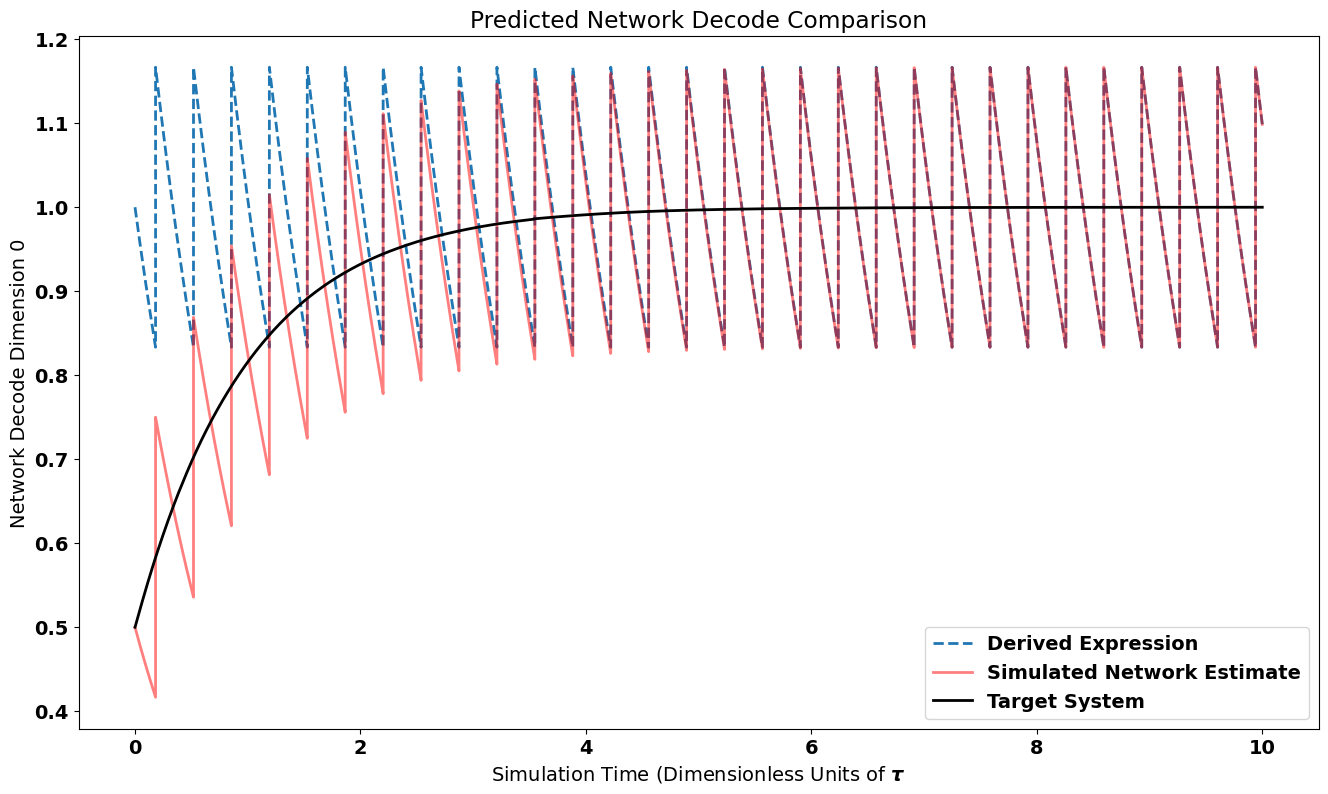
\includegraphics[width=\linewidth]{figures/analysis_const_dynamics_const_driving_network_decode_explicit_comparison.png}
\caption{Comparison of the derived long-term network estimate equation (\ref{eq:analysis:constant_driving_constant_dynamics_estimate_equation_explicit}) to numerical simulation. The simulation parameters are described at the beginning of this section, with the decoder matrix $D$ chosen to be the first $d=2$ rows of the N x N identity matrix, scaled by $3$. This ensures the singular value $S_1 = 3$. Using the rate computed by equation (\ref{eq:analysis_const_dynamics_phi_vs_s}), the derived estimate is computed then overlaid on the numerical simulation after offsetting time by the first spike arrival, $\xi_1^1$. }
\label{fig:analysis:constant_driving_constant_dynamics_explicit_vs_simulation_comparison}
\end{figure}



\item Suppose the systems have settled so that equation (\ref{eq:analysis:constant_driving_constant_dynamics_estimate_equation_explicit}) holds. To compute the RMSE of the estimate, consider the interval between two successive spikes. The RMSE over this period is
\begin{equation*}
RMSE_{spike} \overset{\Delta}{=}\
\sqrt
{
	\phi \int_
	{	
		0
	}
	^
	{
		\frac
		{
			1
		}
		{
			\phi
		}
	}
	 \!  e^T e(\tau)\, \, \mathrm{d} \tau
}.
\end{equation*}


Note that the target dynamical system settles to a fixed point $x = \mathcal{U}_1$ so that
\begin{align*}
e(\tau) &= x(\tau) -
 \hat
 {
 	x
 }
 (
 	\tau
 )
%
\\
\\
%
&= 
\mathcal{U}_1 - 
\left(
	1 + 
	\frac
	{
		1
	}
	{
		2 \, S_1
	}
\right)
e^
{
	- \tau
}
\, \, \mathcal{U}_1
%
\\
\\
%
&= 
\mathcal{U}_1 
\left[
	1 - e^
	{
		-\tau
	}
	\left(
		1 + 
		\frac
		{
			1
		}
		{
			2 \, S_1
		}
	\right)
\right]
%
\\
\\
%
\implies
e^T e
\left(
\tau
\right)
&=
\left[
	1 - e^
	{
		-\tau
	}
	\left(
		1 + 
		\frac
		{
			1
		}
		{
			2 \, S_1
		}
	\right)
\right]^2
%
\\
\\
%
&= 
1 - 2 \, e^
{
	-\tau
}
\left(
	1 + 
	\frac
	{
		1
	}
	{
		2 \, S_1
	}
\right)
+
e^
{
	-2 \, \tau
}
\left(
	1 + 
	\frac
	{
		1
	}
	{
		S_1
	}
	+
	\frac
	{
		1
	}
	{
		4 \, S_1^2
	}
\right).
\end{align*}
The integral is therefore 

\begin{align*}
	\int_
	{	
		0
	}
	^
	{
		\frac
		{
			1
		}
		{
			\phi
		}
	}
	 \!  e^T e(\tau)\, \, \mathrm{d} \tau 
	 &= 
	 \frac
	 {
	 	1
	 }
	 {
	 	\phi
	 }
	 -
	 2
	 \left(
	 	1 + 
	 	\frac
	 	{
	 		1
	 	}
	 	{
	 		2 \, S_1
	 	}
	 \right)
	\frac
	{
		\frac
		{
			1
		}
		{
			2
		}
		+ v_{th}
	}
	{
		S_1 + 
		\frac
		{
			1
		}
		{
			2
		}
	}
	+
	\frac
	{
		1
	}
	{
		2
	}
	\left(
		1 + 
		\frac
		{
			1
		}
		{
			S_1
		}
		+
		\frac
		{
			1
		}
		{
			4 \, S_1^2
		}
	\right)
	\left(
		1 - 
		e^
		{
			\frac
			{
				2
			}
			{
				\phi
			}
		}		
	\right)
	%
	\\
	\\
	%
	&= 
	 \frac
	 {
	 	1
	 }
	 {
	 	\phi
	 }
	 -
	 2
	 \frac
	 {
	 	1
	 }
	 {
	 	S_1
	 }
	 \left(
	 	S_1 + 
	 	\frac
	 	{
	 		1
	 	}
	 	{
	 		2
	 	}
	 \right)
	\frac
	{
		\frac
		{
			1
		}
		{
			2
		}
		+ v_{th}
	}
	{
		S_1 + 
		\frac
		{
			1
		}
		{
			2
		}
	}
	+
	\frac
	{
		1
	}
	{
		2
	}
	\left(
		1 + 
		\frac
		{
			1
		}
		{
			S_1
		}
		+
		\frac
		{
			1
		}
		{
			4 \, S_1^2
		}
	\right)
	\left(
		1 - 
		e^
		{
			\frac
			{
				2
			}
			{
				\phi
			}
		}		
	\right)
		%
	\\
	\\
	%
	&= 
	 \frac
	 {
	 	1
	 }
	 {
	 	\phi
	 }
	 -
	 \frac
	 {
	 	1 + 2\, v_{th}
	 }
	 {
	 	S_1
	 }
	+
	\frac
	{
		1
	}
	{
		2
	}
	\left(
		1 + 
		\frac
		{
			1
		}
		{
			S_1
		}
		+
		\frac
		{
			1
		}
		{
			4 \, S_1^2
		}
	\right)
	\left(
		1 - 
		e^
		{
			\frac
			{
				2
			}
			{
				\phi
			}
		}		
	\right),
	%
	\\
	\\
	%
	&= 
	 \frac
	 {
	 	1
	 }
	 {
	 	\phi
	 }
	 -
	 \frac
	 {
	 	1 + 2\, v_{th}
	 }
	 {
	 	S_1
	 }
	+
	\frac
	{
		1
	}
	{
		2
	}
	\frac
	{
		1
	}
	{
		S_1
	} 
	\left(
		1 + 
		\frac
	{
			1
		}
		{
			4 \, S_1
		}
		+ 
		2\, v_{th}
		-
		\frac
		{
			v_{th}^2
		}
		{
			S_1
		}
	\right)
	%
	\\
	\\
	%
	&= 
	\frac
	{
		1
	}
	{
		\phi
	}
	-
	\frac
	{
		1 + 2 \, v_{th} -
		\frac
		{
			1
		}
		{
			S_1
		}
		\left(
			\frac
			{
				1
			}
			{
				4
			}
			- v_{th}^2
		\right)
	}
	{
		2 \, S_1
	}	
	%
	\\
	\\
	%
	&= 
	\frac
	{
		1
	}
	{
		\phi
	}
	- \frac
	{
		1
	}
	{
		S_1
	},
\end{align*}
where we have used the earlier result
\begin{align*}
\frac
{
	S_1^
	{
		-1
	}
}
{
	1 - e^
	{
		\frac
		{
			1
		}
		{
			\phi
		}
	}
}
&= 
1 + 
\frac
{
	1
}
{
	2 \, S_1
},
\end{align*}
and 
\begin{align*}
	e^
	{
		-
		\frac
		{
			2
		}
		{
			\phi
		}
	}
	&= 
	\frac
	{
		\left(
			1 - \frac
			{
				v_{th}
			}
			{
				S_1
			}
		\right)^2
	}
	{
		\left(
			1 + \frac
			{
				1
			}
			{
				2 S_1
			}
		\right)^2
	}
	%
	\\
	\\
	%
	&= 
	\frac
	{
		1 
		-
		2 \, \frac
		{
			v_{th}		
		}
		{
			S_1
		}
		+
		\frac
		{
			v_{th}^2
		}
		{
			S_1^2
		}
	}
	{
		1 + 
		\frac
		{
			1	
		}
		{
			S_1
		}
		+
		\frac
		{
			1
		}
		{
			4 \, S_1^2
		}	
	}
	%
	\\
	\\
	%
	\implies
	1 - e^
	{
		-\frac
		{
			2
		}
		{
			\phi
		}
	}
	&= 
	\frac
	{
			1 + 
		\frac
		{
			1	
		}
		{
			S_1
		}
		+
		\frac
		{
			1
		}
		{
			4 \, S_1^2
		}
		- 1
		+ 2 \, 
		\frac
		{
			v_{th}
		}
		{
			S_1
		}	
		-\frac
		{
			v_{th}^2
		}
		{
			S_1^2
		}
	}
	{
			1 + 
		\frac
		{
			1	
		}
		{
			S_1
		}
		+
		\frac
		{
			1
		}
		{
			4 \, S_1^2
		}	
	}
	%
	\\
	\\
	%
	&=
	\frac
	{
		\frac
		{
			1
		}
		{
			S_1
		} 
		\left(
			1 + 
			\frac
			{
				1
			}
			{
				4 \, S_1
			}
			+ 
			2\, v_{th}
			-
			\frac
			{
				v_{th}^2
			}
			{
				S_1
			}
		\right)
	}
	{
		1 + 
		\frac
		{
			1	
		}
		{
			S_1
		}
		+
		\frac
		{
			1
		}
		{
			4 \, S_1^2
		}		
	}.
\end{align*}

Consequently the per-spike RMSE of the network estimate is given by 
\begin{align}
\label{eq:analysis:const_dynamics_per_spike_rmse_phi_s}
RMSE_{spike}(s, \phi(s)) = \sqrt
{
	1 - 
	\frac
	{
		\phi
	}
	{
		S_1
	}
}.
\end{align}
To write the above equation as a function of only $\phi$, we invert equation (\ref{eq:analysis_const_dynamics_phi_vs_s}) to obtain 
\begin{align}
\label{eq:analysis:const_dynamics_per_spike_rmse_phi}
S_1(\phi) &= 
\frac
{
	v_{th} +
	\frac
	{
		e^
		{
			-\frac
			{
				1
			}
			{
				\phi
			}
		}
	}
	{
		2
	}
}
{
	1 - e^
	{
		-\frac
		{
			1
		}
		{
			\phi
		}
	}
}
\notag
%
\\
\notag
\\
%
\implies
RMSE_{spike} 
&= 
\sqrt
{
	1 - \phi 
	\left(
		\frac
		{
			1 - e^
			{
				-\frac
				{
					1	
				}
				{
					\phi
				}
			}
		}
		{
			v_{th} + 
			\frac
			{
				1
			}
			{
				2
			}
			e^
			{
				-\frac
				{
					1
				}
				{
					\phi
				}
			}
		}
	\right)
} \notag
%
%
\\  
\notag
\\
\notag
%
%
&= 
\sqrt
{
	1 + 2 \phi 
	\left(
		\frac
		{
			e^
			{
				-\frac
				{
					1	
				}
				{
					\phi
				}
			}
			- 1
		}
		{
			e^
			{
				-\frac
				{
					1
				}
				{
					\phi
				}
			}
			+ 1
		}
	\right)
}
\notag
%%
%%
\\
\notag
\\
%%
%%
&=\sqrt
{
	1 - 2 \phi
	\tanh
	{
		\frac
		{
			1
		}
		{
			2 \, \phi
		}	
	}
}.
\end{align}

The preceding equation is plotted in figure (\ref{fig:analysis:const_dynamics_per_spike_rmse_vs_phi_s}). Above spikes rates of $\phi = 1$, the relationship is linearly decreasing on a logarithmic scale.
%\begin{align*}
%	\frac
%	{
%		\mathrm{d} RMSE_{spike}
%	}
%	{
%		\mathrm{d} \phi
%	}
%	%%%%%%%%%%%
%	%%%%%%%%%%%
%	&= 
%	%%%%%%%%%%%
%	%%%%%%%%%%%
%	\frac
%	{
%		\phi
%	}
%	{
%		2
%	}
%	\frac
%	{
%		-\frac	
%		{
%			e^
%			{
%				-
%				\frac
%				{
%					1
%				}
%				{
%					x
%				}
%			}
%		}
%		{
%			x^2
%		}
%		\frac
%		{
%			1
%		}
%		{
%			2
%		}
%		\left(
%			1 + e^
%			{
%				-\frac
%				{
%					1
%				}
%				{
%					\phi
%				}
%			}
%		\right)
%		-
%				-\frac	
%		{
%			e^
%			{
%				-
%				\frac
%				{
%					1
%				}
%				{
%					x
%				}
%			}
%		}
%		{
%			2 \, x^2
%		}
%		1 - e^
%		{
%			-\frac
%			{
%				1
%			}
%			{
%				\phi
%			}
%		}
%	}
%	{
%		\sqrt
%		{
%			1 - \phi
%			\left(
%				\frac
%				{
%					1 - e^
%					-\frac
%					{
%						1
%					}
%					{
%						\phi
%					}
%				}
%				{
%					\frac
%					{
%						1
%					}
%					{
%						2
%					}
%					\left(
%						1 + e^
%						{
%							-\frac
%							{
%								1
%							}
%							{
%								\phi
%							}
%						}
%					\right)
%				}
%			\right)
%		}
%	}
%\end{align*}
% To verify this intuition, assume $\phi$ is sufficiently large so that $\frac{1}{\phi}$ is close to $0$. Then we use the approximation,  $e^{x} \simeq 1 + x$ to obtain
%\begin{align*}
%\frac
%{
%	1 - e^
%		{
%			-\frac
%			{
%				1
%			}
%			{
%				\phi
%			}
%		}
%}
%{
%	v_{th} + \frac
%	{
%		1
%	}
%	{
%		2
%	}
%	e^
%	{
%		-\frac
%		{
%			1
%		}
%		{
%			\phi
%		}
%	}
%}
%\simeq
%\frac
%{
%	1 - 
%	\left(
%		1 + 
%		\frac
%		{
%			1
%		}
%		{
%			\phi
%		}
%	\right)
%}
%{
%	v_{th} +
%	\frac
%	{
%		1
%	}
%	{
%		2
%	}	
%	\left(
%		1 + 
%		\frac
%		{
%			1
%		}
%		{
%			\phi
%		}
%	\right)
%}
%%
%\\
%\\
%%
%&= 
%\frac
%{
%	1
%}
%{
%	\phi
%	\left(
%		1 + 
%		\frac
%		{
%			1
%		}
%		{
%			2 \, \phi
%		}
%	\right)
%}
%%
%\\
%\\
%%
%&=
%\frac
%{
%	1
%}
%{
%	\left(
%		\phi + \frac{1}{2}
%	\right)
%}
%%
%\\
%\\
%%
%\implies
%RMSE_{spike} \simeq \sqrt
%{
%	1 - 
%}
%\end{align*}

\begin{figure}
\centering
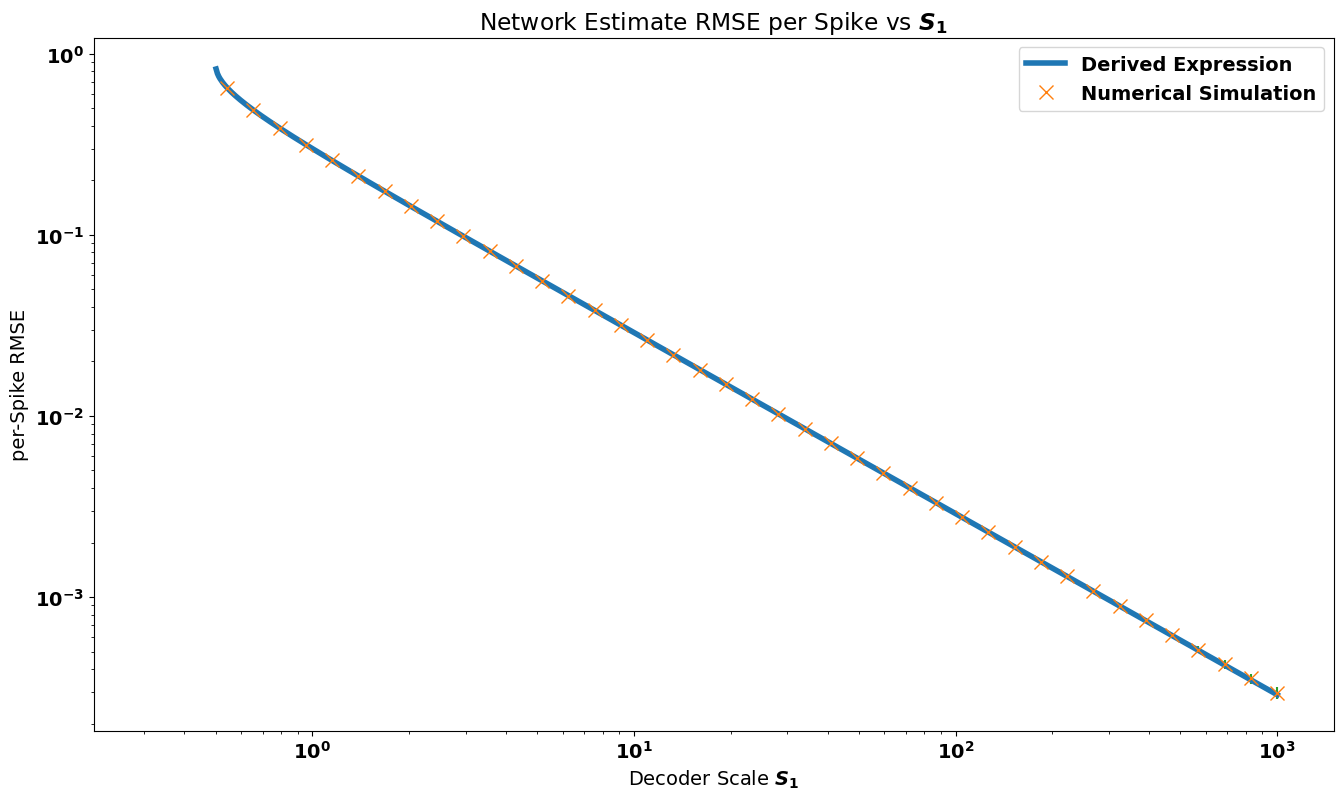
\includegraphics[width=\linewidth]{figures/rmse_sp_vs_s_const_driving.png}
\centering
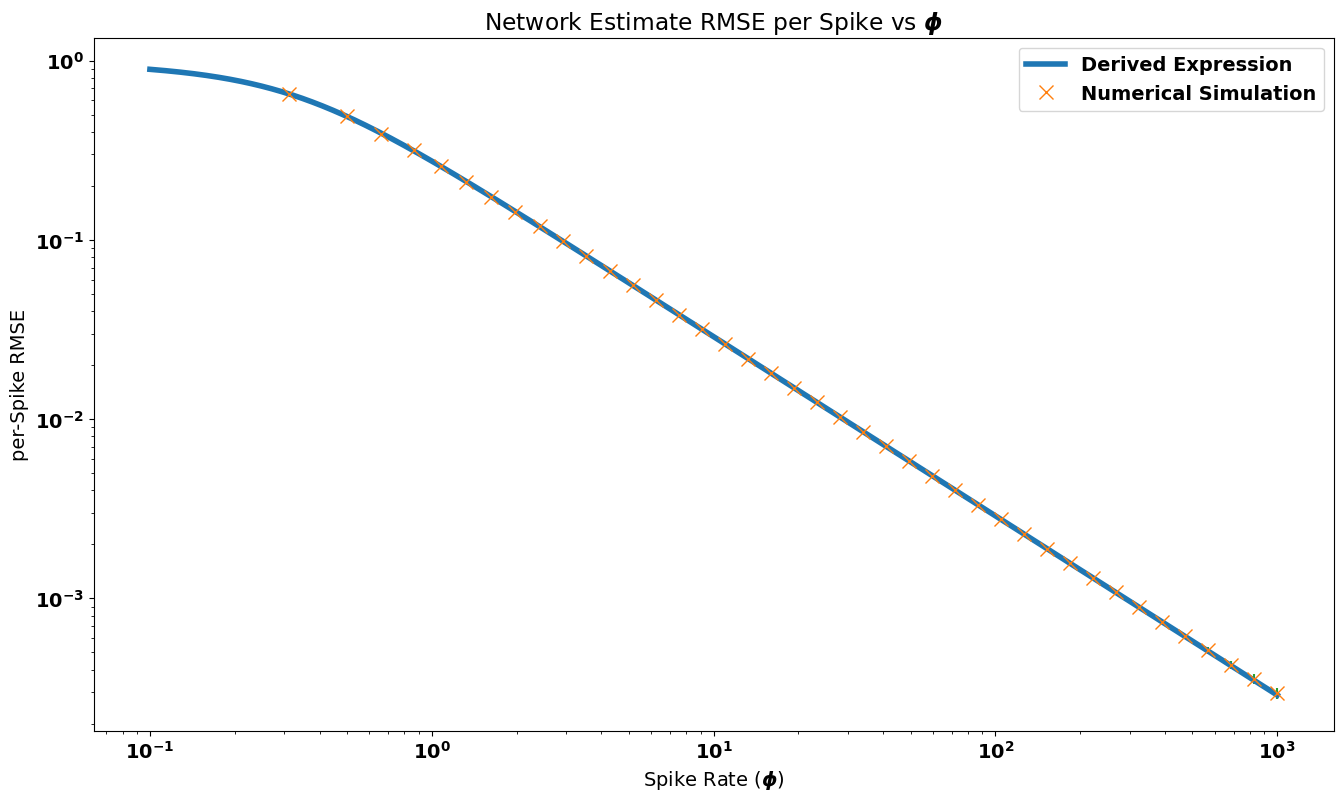
\includegraphics[width=\linewidth]{figures/rmse_sp_vs_phi_s_const_driving.png}
\caption{\textbf{\textit{Top:}} A log-log plot of equation (\ref{eq:analysis:const_dynamics_per_spike_rmse_phi_s}) compared with numerical measurements.  \textbf{\textit{Bottom:}} A log-log plot of equation (\ref{eq:analysis:const_dynamics_per_spike_rmse_phi}).
\textbf{\textit{Both:}} Each simulated data point is the RMSE averaged over all inter-spike intervals in a simulation of length $T = 80 \tau_s$ with $d\xi = 10^{-4}$. Green vertical lines visible towards the larger values are +/- 1 standard deviation over the number of inter-spike intervals in a given simulation. The spike rates $\hat{\phi}$ were computed numerically via dividing the number of spikes in a simulation by the simulation duration. The RMSE between two adjacent spikes was computed by numerical integration as a discrete sum: $\hat{RMSE} = \sqrt{\hat{\phi} \sum_{\tau \text{ between spikes }} e(\xi)^T e(\xi) \, \, d\xi }$.}
\label{fig:analysis:const_dynamics_per_spike_rmse_vs_phi_s}
\end{figure}


 





\end{enumerate}




































